\section{Methodology}
\label{sec}

\subsection{Data Collection}
\label{subsec:data_collection}
The dataset used in this research is based on the ITC2007 Track 3: Curriculum-Based Course Timetabling (CB-CTT). This dataset has instances where it contains detailed information. This information include a header and four main sections: courses, rooms, curricula, and constraints, with each section containing arrays corresponding to a specific component in the problem and all scalar values summarised in the header. Each dataset instance provides the basic information for testing and validating the proposed approach. 

\begin{figure}[] % h stands for 'here'
    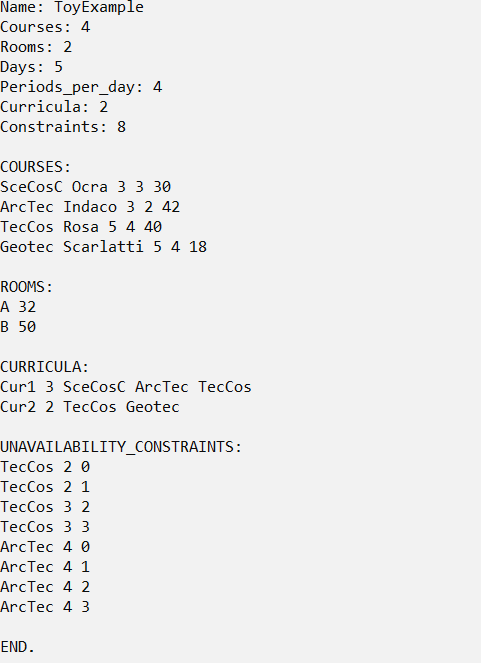
\includegraphics[width=1\textwidth]{example.png}
    \caption{Example of CB-CTT Instance}
    \label{fig:example} % label for referencing
\end{figure}

\clearpage

The header describes the important properties of the instance: name of the instance, number of courses, rooms, working days, periods per day, curricula, and constraints. These values determine the scope and size of the timetabling problem and the boundaries of feasible scheduling.

In the \textbf{Courses} section, every course is specified to include the assigned teacher, number of lectures required, minimum number of working days that lectures should be spread, and number of students enrolled. 

The \textbf{Rooms} section defines the rooms available for scheduling along with their seating capacities. 

Under \textbf{Curricula}, the courses of similar curricula are combined together such that no two classes from a particular curriculum fall at the same time. 


The \textbf{Unavailability Constraints} section specifies day-period combinations during which certain courses cannot be scheduled. These constraints typically arise from limitations such as teacher unavailability or room restrictions. 

This structured dataset gives a stable base for testing and verification of the proposed MPSO, thus ensuring that all the constraints imposed on it are well described.

\subsection{Data Processing}
\label{subsec:data_processing}

The data processing phase transforms the raw dataset into a structured and optimized format suitable for integration into the MPSO framework. All problem components and constraints are accurately represented to allow seamless initialization of particles and candidate solution evaluation.

The dataset contains courses, rooms, curricula, and unavailability constraints, which are parsed and normalized in order to achieve consistency. Time-related data, that is, days and periods, are converted to numerical indices, and the constraints are encoded to lead the process of optimization. The parsed data is structured into a particle representation, that is, encoding each candidate solution of the timetabling problem as a list of scheduling entries in the format:

\[
(\text{Day}, \text{Period}, \text{Room}, \text{Course}).
\]

\subsubsection*{Constraint Encoding}

The constraints, central to the problem, can be categorized into two types, namely hard constraints and soft constraints. Hard constraints are mandatory and must be strictly satisfied, while soft constraints are desirable properties that contribute to the overall quality of the solution. The details and mathematical representations of these constraints are given as follows:

\clearpage

\begin{table}[h]
    \centering
    \begin{tabular}{|c|p{10cm}|}
    \hline
    \textbf{Symbol} & \textbf{Definition} \\ \hline
    \(d, p, r, c\) & Day, Period, Room, and Course respectively. \\ \hline
    \(S\) & Set of all scheduling entries, where each entry is \((d, p, r, c)\). \\ \hline
    \(U\) & Set of unavailability constraints, specifying unavailable periods for certain courses. \\ \hline
    \(\operatorname{Curr}(k)\) & Set of courses in curriculum \(k\). \\ \hline
    \(T(c)\) & Teacher assigned to course \(c\). \\ \hline
    \(\text{students}(c)\) & Number of students enrolled in course \(c\). \\ \hline
    \(\text{capacity}(r)\) & Capacity of room \(r\). \\ \hline
    \(\text{min\_days}(c)\) & Minimum number of days required for course \(c\). \\ \hline
    \(R_c\) & Set of rooms assigned to course \(c\) across all scheduled periods. \\ \hline
    \end{tabular}
    \caption{Symbols used for the CB-CTT problem}
    \label{tab:symbols}
\end{table}

\paragraph*{Hard Constraints}

\begin{enumerate}
    \item \textbf{Lecture Assignment}:
    Each lecture of a course must be assigned to a unique combination of day, period, and room. Overlaps are strictly prohibited.
    \[
    \forall (d, p, r, c_i), (d', p', r', c_j) \in S, \quad i \neq j \Rightarrow (d, p, r) \neq (d', p', r').
    \]

    \item \textbf{Room Occupancy}:
    No two lectures can occupy the same room at the same time.
    \[
    \forall (d, p, r, c_i), (d, p, r, c_j) \in S, \quad i \neq j \Rightarrow c_i \neq c_j.
    \]

    \item \textbf{Conflicts}:
    Courses in the same curriculum or taught by the same teacher must not overlap in time.
    \[
    \forall (d, p, r, c_i), (d, p, r', c_j) \in S, \quad (c_i \in \operatorname{Curr}(k) \lor T(c_i) = T(c_j)) \Rightarrow p_i \neq p_j.
    \]
    Here, \(\operatorname{Curr}(k)\) represents the courses in curriculum \(k\), and \(T(c)\) is the teacher assigned to course \(c\).

    \item \textbf{Availability}:
    Courses cannot be scheduled during unavailable periods as specified in the dataset.
    \[
    \forall (c, d, p) \in U, \quad (d', p', r, c') \in S, \quad c' = c \Rightarrow (d' \neq d \lor p' \neq p).
    \]
\end{enumerate}

\paragraph*{Soft Constraints}

\begin{enumerate}
    \item \textbf{Room Capacity}:
    Assigning a course to a room with insufficient capacity incurs a penalty proportional to the seating deficit.
    \[
    P_1 = \sum_{(d, p, r, c) \in S} \max(0, \operatorname{students}(c) - \operatorname{capacity}(r)).
    \]

    \item \textbf{Minimum Working Days}:
    Scheduling a course for fewer days than its minimum requirement results in a penalty.
    \[
    P_2 = \sum_{c \in C} 5 \cdot \max(0, \operatorname{min\_days}(c) - |\{d \mid (d, p, r, c) \in S\}|).
    \]

    \item \textbf{Room Stability}:
    Assigning a course to multiple rooms across its schedule incurs a penalty for each additional room used.
    \[
    P_3 = \sum_{c \in C} \max(0, |R_c| - 1), \quad R_c = \{r \mid (d, p, r, c) \in S\}.
    \]

    \item \textbf{Curriculum Compactness}:
    Isolated lectures for a curriculum within a day are penalized, promoting schedule compactness.
    \[
    P_4 = \sum_{k} \sum_{d} \sum_{p \in P_d} \operatorname{is\_isolated}(p),
    \]
    where \(\operatorname{is\_isolated}(p) = 2\) if no adjacent lectures exist for curriculum \(k\).
\end{enumerate}

\subsubsection*{Fitness Function}

The overall fitness function integrates the penalties for soft constraints and serves as the objective function for optimization. It is expressed as:
\[
\text{Fitness} = P_1 + P_2 + P_3 + P_4.
\]

\subsubsection*{Validation and Testing}

The parsed data is verified for completeness and consistency during the process. It checks to ensure that all courses, rooms, and curricula have been represented accurately and the constraints are correctly encoded. Thus, the structured and validated data forms a robust base for initializing particles and guiding the optimization process.

The approach of comprehensive data processing will prepare the problem constraints and components for the MPSO framework in an accurate manner so that hard constraints are maintained and soft constraint penalties are optimized.

\subsection{Approach Construction}
\label{subsec:approach_construction}
The approach begins with initializing particles in the Multi-Swarm Particle Swarm Optimization (MPSO) algorithm. Each particle represents a potential solution—a timetabling configuration. 
1. **Initialization**: Particles are initialized using heuristic methods like Largest Degree (LD), ensuring an initial feasible solution that respects hard constraints.
2. **Optimization Loop**: The MPSO iteratively improves solutions by updating particle positions and velocities based on personal best and global best configurations.
3. **Diversity Mechanisms**: The algorithm employs exclusion, anti-convergence, and quantum reinitialization mechanisms to maintain diversity and prevent premature convergence.
4. **Fitness Evaluation**: Each particle’s fitness is computed based on a composite objective function incorporating penalties for violations of both hard and soft constraints.

\subsection{Approach Evaluation}
\label{subsec:approach_evaluation}
The performance of the MPSO algorithm is validated against the ITC2007 datasets. The evaluation process includes:
- **Validation Tool**: A provided executable from ITC2007 is used to evaluate the feasibility and quality of the generated timetable.
- **Metrics**: Hard constraint violations are strictly penalized, while soft constraint violations contribute to the overall cost. The fitness function aims to minimize this cost.
- **Comparison**: The proposed algorithm is benchmarked against existing methods to highlight its effectiveness in generating high-quality timetables.

\subsection{Deployment}
\label{subsec:deployment}
The final solution is implemented as a web-based application using the Streamlit Python framework. This interface allows users to upload dataset files, run the MPSO algorithm, and generate optimized timetables. The application outputs the timetable in a user-friendly format and provides a summary of the solution's quality, including constraint violations and overall cost.
